\section{Plasma}
	\label{sec:plasma}
	This section presents a short overview of basic plasma theory, it can serve as a
	quick reminder if already familiar with the subject, and necessary
	background to understand the numerical simulations in this work.
    % If you, the reader, is already familiar with plasma physics this section could serve as
    % as a quick reminder about important basic plasma theory. Or it could hopefully
    % serve as a too short and shallow introduction, to the uninitatied reader,
    % of the knowledge needed to make sense of the numerical experiments in this
    % thesis.
	For a more thorough introduction the books \textit{\citetitle{fitzpatrick_plasma_2014}}
    \citep{fitzpatrick_plasma_2014}, \textit{\citetitle{goldston_introduction_1995}} \citep{goldston_introduction_1995},
    \textit{\citetitle{pecseli_waves_2012}} \citep{pecseli_waves_2012} or the classic
    \textit{\citetitle{chen_introduction_1984}} \citep{chen_introduction_1984} can be consulted.

	Plasma is the fourth, lesser known, state of matter. It is similar to a gas
	in the the particles are free to move, but it has the key distinction that
	a proportion of its constituent particles are electrically charged.
	\\[1.0cm]
	\indent \textit{\large"A plasma is a quasineutral gas of charged and neutral particles which exhibits
	collective behaviour."}
	\begin{flushright}
	    \textbf{Francis F. Chen}\\[1.0cm]
	\end{flushright}
	The charge causes the particles to be subject to the Lorentz force, \cref{eq:lorentz}, which
	changes the behaviour of the gas. The plasma state is a typical state,
	sun/stars, northen light, plasma cutters (Welding arcs), argon light tubes, fusion, a lot of various
	industrial techniques, earth athmosphere. (Make this into a paragraph)

	Plasma are fun because of (Intriguing physics, useful for industrial applications,
	solar storms, the ever elusive fusion, space craft, predicting solar storms)

	\begin{figure}
		\begin{center}
			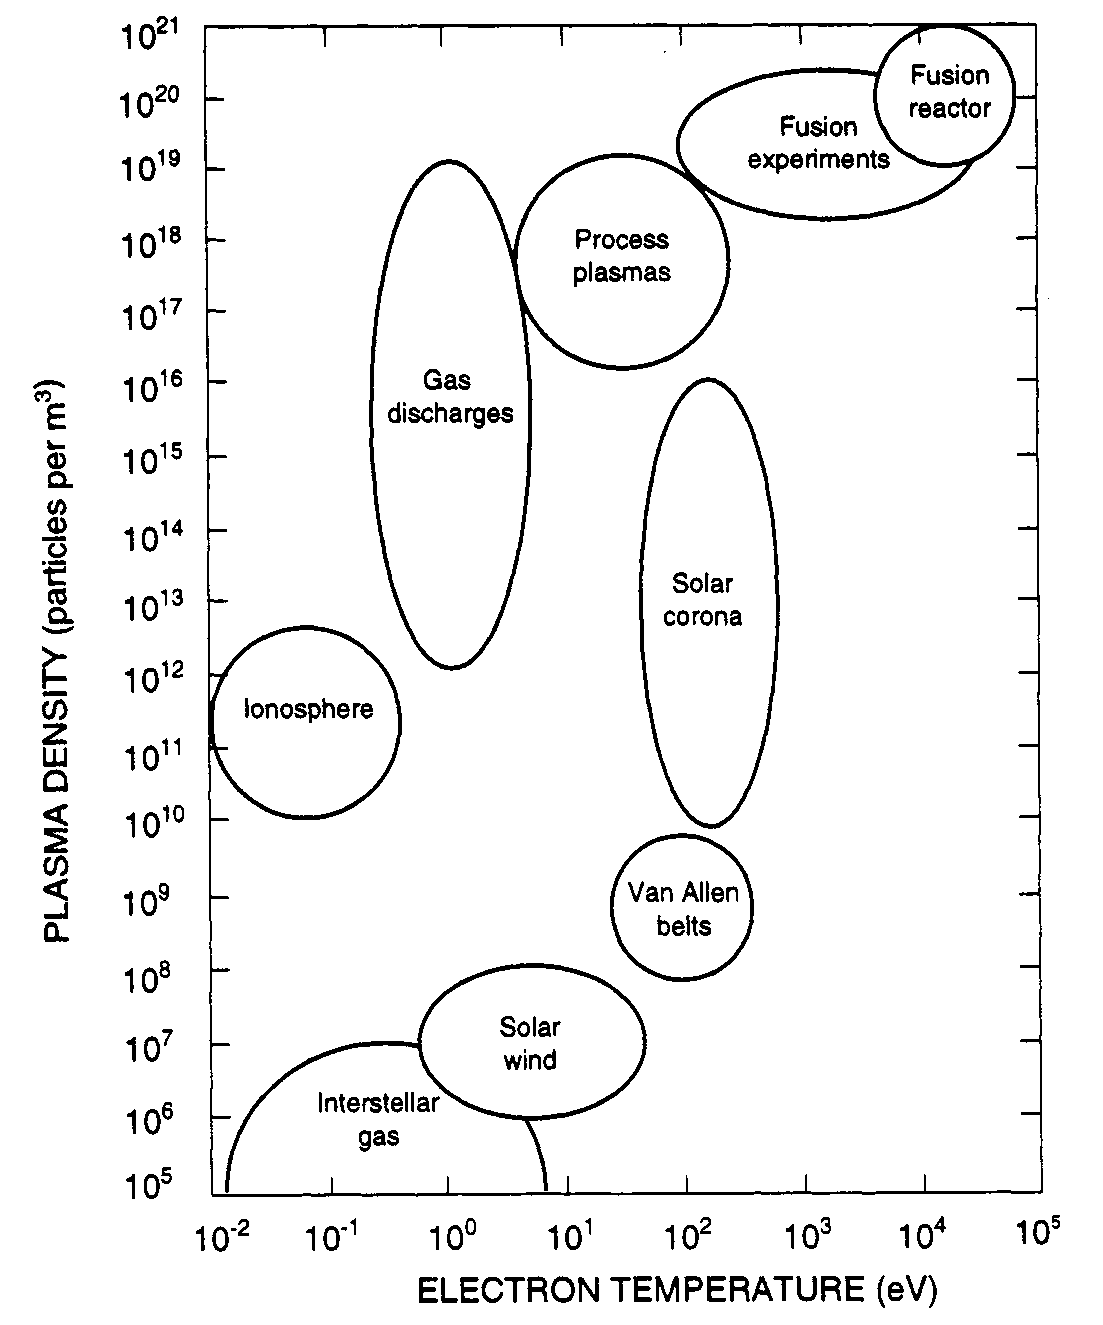
\includegraphics[width = 0.5\textwidth]{figures/theory/plasma_density}
		\end{center}
		\caption{Plasmas occurs both in the hot and dense condiotions in necessary for fusion, as
		well as in the cold and sparse interstellar environment. [NOTE MAKE BETTER FIGURE]
		}
	\end{figure}



    \subsection{Plasma Parameters}
		\label{sec:parameters}

		\subsubsection{Electron Plasma Frequency}

		\begin{itemize}
			\item Slab oscillating, plasma frequency falls out
		\end{itemize}

		\begin{equation}
			\omega_{pe} \equiv \sqrt{\frac{ne^2}{\epsilon_0 m_e}}
		\end{equation}

		\begin{equation}
			\tau_p \equiv 2\pi/\omega_{pe}
		\end{equation}

		\subsubsection{Debye Shielding}
		Debye shielding is heuristically the distance at which the electric influence
		from a particle is shielded out by the surrounding plasma.
		Consider a charged particle immersed in a plasma bath. The plasma is in
		a thermodynamically equilibrium, i.e. there is no significant temperature
		gradients.



		\begin{equation}
			\lambda_D \equiv \sqrt{\frac{\epsilon_0 T}{n e^2}}
		\end{equation}

		\subsubsection{Quasineutrality}
		The assumption of quasi-neutrality is often a valid approximation in plasma
		physics. By quasi-neutrality we assume that we in the analysis set the electron
		density equal to the electron density, \(n_e \approx n_i\). This is often called the
		\textit{"plasma approximation"}, \citep{chen_introduction_1984}. This approximation is often valid on scales
		much larger than the Debye length due to the following arguement. If a
		large volume of plasma lost a significant amount of charge a large electric
		field accompany the density imbalance. This electric field would quickly correct
		the imbalance.

		\subsubsection{Thermal speed}

		\citet{goldston_introduction_1995}

		\subsubsection{TBR(emoved)}
        Let us first consider an idealized plasma, with approximately equal number
        of ions and electrons. Each of the species has mass \(m_s\), where the
        subscript, \(_s\), signifies specie, and respectively charge \(-e, \; +e\). Then we let the plasma be in a quasi-neutral state
        so the number density, \(n\), is apprimately equal, \(n_i\approx n_e = n\).
        Now let's introduce the concept of kinetic temperature \(T_s\), i.e. the random
        motion of the kinetic energy.

        \[T_s \equiv \frac{1}{3}m_s \left< v_s^2 \right> \]

        With the kinetic temperature we define the thermal speed, \(v_{ts}\), as

        \[ v_{ts} \equiv \sqrt{2T_s}/m_s \]

        here we should note that the electron thermal speed is usually much larger
        than the ion thermal speed due to the mass proportion between them.

        Time scales in plasma is usually related to the plasma frequency, \(\omega_{pe}\), of the
        electron as the fastest gyrating particle.

        The reciprocal of the plasma frequency, the plasma period,  is often
        helpful as well.

        Then we define the Debye length \(\lambda_D\) as the length a typical particle
        travels in a plasma period, ignoring the ion contribution.



		\subsubsection{Plasma Classification}
        For a plasma description to be useful the system we consider must have
        a typical length scale, \(L\), and time scale, \(\tau\), larger than the Debye length and plasma
        period respectively.

        \[\frac{\lambda_D}{L} \ll 1  \qquad{} \qquad \frac{\tau_p}{\tau} \ll 1 \]


















%Stay here fucker
